\documentclass{sysuthesis}



%题目
\title{基于压缩文本的字符串近似查询算法研究}
%作者
\author{李贝瑀}
%院系
\school{数据科学与计算机学院}
%专业
\major{计算机科学与技术}
%学生
\student{李贝瑀}
%学号
\studentid{11318030}
%指导教师
\mentor{林瀚(讲师)}
%日期
\date{二〇一六年四月}



%开题报告正文
\openingrep{
	选题目的\\
	如何高效的存储大量字符串以及快速检索其中相近的子集,在基因组序列、Wiki条目等问题中起着关键的作用。目前较多的方法只侧重于其中一点,即牺牲查找速度实现压缩存储,或建立大规模的索引加快搜索。因此,找出一种兼备存储效率及检索速度的方法很有实用意义。\\
	\\
	思路及方法\\
	对于文本压缩,比较常见的方法是对于某些近似的字符串,选出一个字符串作为它们的参考。该方法的问题在于,对于需要检索的字符串,只能找出与其近似的参考,而不是近似的字符串子集。
	在这个方法的基础上加以改进,我们可以构建分层结构的多重参考,即每个字符串存在多个参考,参考间存在层次化的依赖关系。对于检索,需要先找到匹配的参考,通过对参考中预处理信息的考察,得出所有与询问串编辑距离小于k的字符串集合。
	问题的难点在于,找出合适的算法与数据结构,用于构造字符串间的参考关系,在保证较高压缩率的同时,兼顾检索的速度。\\
	\\
	进度安排\\
	2015年12月 查看文献,总结他人在该类问题上的思路与技巧\\
	2016年03月 尝试多种算法及数据结构,测试比较并完成论文撰写\\
}

%开题报告指导教师意见
\openingopinion{
	海量数据的存储和检索是数据科学的重要问题,作者的选题有学术价值,也有技术难度。\\
}



%第一次过程检查的学生总结
\firstcheck{
	阅读了几篇关于字符串压缩、字符串k近似匹配的论文,学习解决这两个问题较为常见的思路、方法。
}
%第一次过程检查的指导老师意见
\firstopinion{先实现已有的算法,对比试验结果,再继续深入研究、实现复杂的策略并改善原有的策略。}
%第二次过程检查的学生总结
\secondcheck{
	大致构建了压缩的算法、查询的算法框架,考虑用后缀数组或者后缀树做字符串匹配。\\
	从部分结果进行扩展时,似乎可以使用函数式线段树查询区间,但空间复杂度略高。
}
%第二次过程检查的指导老师意见
\secondopinion{修改部分算法的实现形式,通过实验找出最合适的算法。}
%第三次过程检查的学生总结
\thirdcheck{
	最终选择了较为简洁的后缀自动机作为主要的数据结构进行字符串匹配,区间的查询可用区间树维护。\\
	完成了总体的代码,压缩率一般,继续考虑较为细节的策略。
}
%第三次过程检查的指导老师意见
\thirdopinion{可针对不同数据类型进行实验,以此寻找改进的策略。}
%整体完成情况的指导老师意见
\overallopinion{\rule{0cm}{4\baselineskip}}



%指导教师评语
\instructorcomment{\rule{0cm}{6\baselineskip}}
%指导教师给予的成绩评定
\instructorgrade{\rule{0cm}{2\baselineskip}}
%答辩小组或专业负责人意见
\majorcomment{\rule{0cm}{4\baselineskip}}
%答辩小组或专业负责人给予的成绩评定
\majorgrade{\rule{0cm}{2\baselineskip}}
%院系负责人意见
\schoolcomment{\rule{0cm}{3\baselineskip}}
%院系负责人给予的成绩评定
\schoolgrade{\rule{0cm}{2\baselineskip}}



\cabstract{
	对于海量数据的存储与检索,是数据科学领域的重要问题,在构建人类基因库、Wiki文库历史版本维护等问题中起着关键作用。近年来,越来越多的研究开始将两者结合起来,在保证数据压缩存储的同时,兼备检索的能力。本文旨在利用一种较为简洁的数据结构——后缀自动机,对于可添加的字符串集合,动态构建包含多个引用的层次化索引结构,其中:1)引用的选择由程序自身决策,而非人工选择;2)支持基于编辑距离的近似字符串匹配。经证实,对于索引结构的字符串压缩方案来说,寻找空间最优解是一个NP-hard问题。因此,本文的最终目标在于尽量优化存储空间,在满足较高压缩率的同时,兼顾检索的速度。
}
\keywords{数据压缩;近似匹配;索引;后缀自动机}
\eabstract{
	Storing and searching of massive data is an important issue in the field of data science, which plays a key role in problems as construction of the human gene pool and in maintenance problems about historical versions in Wiki library. Recently, more and more researchers have been beginning to combine them. In other words, when it comes to the compressed storage of data, the searching ability is also demanded. This paper aims to use a relatively compact data structure - suffix automaton, to dynamically build the hierarchical index structure containing multiple reference, for the set of strings that can expand, in which: 1) the reference is selected by its own decision-making procedures, rather than artificial selection; 2) it is supported to match approximate string based on their edit-distance. It was confirmed that for the index structure string compression scheme, finding the optimal solution in space is an NP-hard problem. Therefore, the ultimate goal of this paper is trying to optimize storage space to meet the higher compression ratio while taking a efficent searching method into account.
}
\ekeywords{Compression; approximate matching; indexing; suffix automaton}



\begin{document}

\frontmatter

\cleardoublepage
\tableofcontents

\mainmatter



\chapter{引言}
在信息科学领域中,字符串及相关问题一直以来都是研究的热点,其中最具代表性的当属匹配\cite{knuth1977fast}与压缩\cite{ziv1977universal}问题。在数据量越来越大的今天,直接对字符串本身进行存储将占用大量空间,如何在其中检索有用的信息也是一大难题。那么对于庞大的字符串集合,要如何将其压缩至尽量小的空间,却又可以尽量快的进行检索呢?



\section{背景}
近年来,随着信息技术在基因工程方面的普及,越来越多的DNA序列问题依赖计算机来处理。例如在研究基因突变时,由于突变率较低,必须记录下大量实验数据,再找出其中与原DNA序列近似的片段。其他方面,网络知识库的加速更迭,使得历史版本的存储带来挑战。在Wiki条目中,对于某个名词,可能存在许多类似的别称,需要一种近似检索的策略。\par
在字符串检索领域中有一种较为重要的方式——k近似匹配:在一个字符串集合中,找出与模式串之间编辑距离不超过k的所有子串,其中编辑距离表示将模式串通过插入、修改、删除操作变为目标串的最小修改次数。传统的k近似匹配基本只用到两种方法:1)对于集合内的字符串分别处理;2)将集合内的字符串拼接起来处理。这两种方法的局限性在于,存储所占用的空间至少是所有字符串长度之和。由于自然语言的特性,许多语句之间具有极强的关联性,可以通过其中的某一句话的片段,表达其他句子的部分信息,从而达到压缩存储的目的。因此,越来越多研究开始尝试先选择一些字符串作为索引,再将与之相似的串通过引用进行压缩的方法。此时,k近似匹配变成了两个问题:1)在索引集合中检索;2)找出与该索引串相似的引用串。这种方法的问题在于,只有索引中的匹配是精确的,引用串只是与索引串相似,而非模式串。\par
因此,找出一种将两者结合起来,在保证数据压缩存储的同时,兼备高效检索能力的算法是十分有意义的。



\section{相关成果}
我们首先简单介绍一下前人有关字符串压缩算法的研究成果,以及这一技术在解决各领域有关检索问题时的应用。



\subsection{字符串压缩}
字符串压缩是计算机科学及相关领域的经典问题。一种与本文相关的压缩方式,称为基于引用的压缩算法\cite{deorowicz2011robust, pinho2012green},是将被压缩串替换为由其他串的片段构成的引用序列。压缩率取决于字符串间的相似程度,相似度越高则压缩的效果越好。对于某些基因片段来说,这一比率甚至可以达到1,000:1\cite{wandelt2013fresco}。



\subsection{半结构化文档压缩}
对于倒排文档\cite{claude2011indexes}的压缩一般应用于文本文档的储存中,主要思路是将所有出现的词组用标准压缩方式进行压缩,再基于词组进行索引。该方法对于大多数资料有较高的压缩效率\cite{hoobin2011relative},但并不支持字符串的近似检索。



\subsection{基于特殊领域的索引压缩}
对于字符串集合的管理在生物学中十分重要。最近,越来越多的算法致力于用树形的引用结构压缩基因组,并提供近似搜索的可能\cite{yang2013efficient}。该方法可以达到极高的压缩率\cite{danek2014indexes},但对于大量的长字符串,压缩速度较低。其次,由于检索基于筛选出的特定序列\cite{siren2014indexing},因此会遗漏部分结果。



\section{本文工作}
本文结合了前人的研究结果,尝试构建动态的多引用可搜索索引模型,支持动态扩展的字符串集合,通过多引用提高压缩率,自动决策引用的选择以及提供高效的搜索策略。构建思路的难点在于:1)每次要在原有结构的基础上进行简单修改即可完成更新,需要适合的数据结构;2)每个引用串可以引用多个不同的索引,需要在字符串集合中进行快速匹配,并设计尽量优化空间的选择策略;3)需要快速的k近似匹配算法,以及合适的数据结构维护引用的关系,从而递推出全部结果;4)特殊情况的处理。\par
下面我们将对上述问题依次讨论。



\chapter{压缩与索引}
这里我们介绍多引用索引结构\cite{wandelt2015mrcsi}的具体细节,随后我们建立简单的只通过主引用索引的结构,在此基础上再构建基于DAG(Directed Acyclic Graphs)的层次化引用。



\section{符号定义}
首先我们介绍一下本章节用到的定义及符号表示。\par
一个字符串$s$表示一个关于字符集$\Sigma$的有限序列,长度用$|s|$表示。两个字符串的连接用$s \circ t$表示。从下标$i$开始的长度为$n$的字符串用$s(i, n)$表示,特别的对于长度为$1$的子串(即一个字符)用$s[i]$表示,注意这里的下标从0开始。对于两个字符串$s$与$t$,如果他们之间的编辑距离不超过k,即$s$可以通过至多k次插入、修改、删除操作变为$t$,则称$s$与$t$为k近似,记作$s \sim_{k} t$。\par
对于一个索引,我们用$RME$(Referential Match Entry)来表示,是由$(refid, start, length, mismatch)$组成的元组,其中$refid$是被引用串id,$start$表示起始位置,$length$表示长度,$mismatch$表示失配处的字符,即代表字符串$s_{refid}(start, length) \circ mismatch$。\par
对于一个压缩字符串,我们用$RCS$(Referential Compression Sequence)来表示,同时记录下其中每个$RME$的前缀长度$offset_{i}$。



\section{索引结构}
通常来说,在索引结构的字符串集合中,有一部分字符串是不经压缩直接保存的,称为主引用集合($PREF$)。除此之外,其他字符串都直接或间接使用主引用的子串作为索引,称为压缩集合($COMP$)。\par
需要注意的几点是,这里的主引用集合中可以存在多个字符串。这样的好处在于,由于主引用集合中的子串被引用的概率较高,可以提高压缩率。在储存时,只有主引用直接保存原文,其他字符串只保存$RCS$形式的索引信息。由于主引用集合一般较小,故大部分字符串还是以索引的形式保存的。为了方便实现,一般将主引用集合中的字符串也加入压缩集合中。其次,不是只有主引用才可以作为索引,每个串都可以被引用。这样可以防止主引用集合过于庞大,因为主引用集合是未经压缩的。但必须保证的是,互相之间的引用关系不会形成环。\par
下面,我们来看一个简单索引结构的构建。



\section{简单索引}
在最简单的版本中,每个串都只以主引用作为索引。这里有一个样例,若字符串集合$S = \{s_{1}, s_{2}, ... s_{6}\}$,其中:\par
\hspace{1cm}$s_{1}$ = Aho–Corasick Automaton, $s_{2}$ = Aho/Corasick,\par
\hspace{1cm}$s_{3}$ = Aho/Corasick Automata, $s_{4}$ = Aho/Corasick Automatas,\par
\hspace{1cm}$s_{5}$ = Link-cut Tree, $s_{6}$ = LinkCut Tree.\par
对于$s_{2}$来说,引用$s_{1}$构成的$RCS$序列为$[(1, 0, 3, /), (1, 4, 7, k)]$,因为$s_{2} = s_{1}(0, 3) \circ / \circ s_{1}(4, 7) \circ k$。但对于$s_{5}$来说,这样显然就不合适了。因此,我们选择$s_{1}$与$s_{5}$作为主引用,即$PREF = \{s_{1}, s_{5}\}$。此时我们得到:\par
\hspace{1cm}$comp(s_{1}, \{s_{1}\}) = [(1, 0, 21, n)]$\par
\hspace{1cm}$comp(s_{2}, \{s_{1}\}) = [(1, 0, 3, /), (1, 4, 7, k)]$\par
\hspace{1cm}$comp(s_{3}, \{s_{1}\}) = [(1, 0, 3, /), (1, 4, 16, a)]$\par
\hspace{1cm}$comp(s_{4}, \{s_{1}\}) = [(1, 0, 3, /), (1, 4, 16, a), (1, 8, 0, s)]$\par
\hspace{1cm}$comp(s_{5}, \{s_{5}\}) = [(5, 0, 12, e)]$\par
\hspace{1cm}$comp(s_{6}, \{s_{5}\}) = [(5, 0, 4, C), (5, 6, 6, e)]$\par
他们之间的引用关系如图\ref{image:csimple}所示。\par

\begin{figure}[htbp]
	\centering
	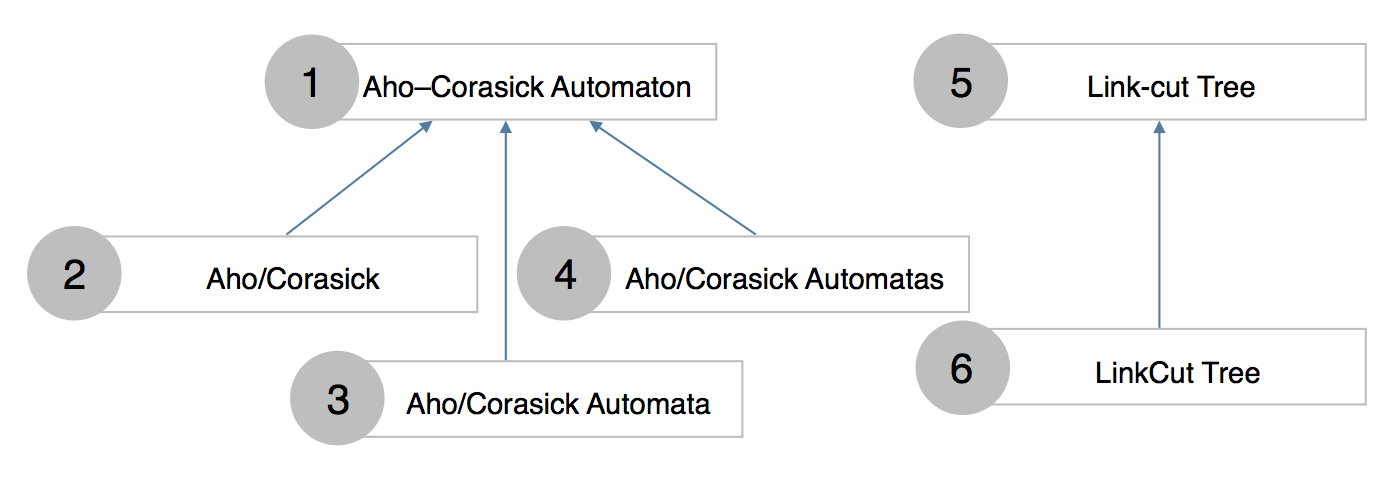
\includegraphics[scale=0.3]{image/csimple.png}
	\caption{简单索引}\label{image:csimple}
\end{figure}

接下来,我们介绍构建的具体算法。\par
在初始状态下,有$PREF = \emptyset$,$COMP = \emptyset$。随后加入$s_{1}$时,由于$PREF$为空,$s_{1}$无法选择任何引用,故将$s_{1}$加入$PREF$,得到$PREF = \{s_{1}\}$,$COMP = \{s_{1}\}$。在加入$s_{2}$时我们有两种选择:1)将$s_{2}$加入$PREF$;2)以$s_{1}$作为引用构建索引。显然,当$s_{1}$与$s_{2}$较为相似时,选择后者较优,这时我们得到$PREF = \{s_{1}\}$,$COMP = \{s_{1}, s_{2}\}$。否则选择前者,此时$PREF = \{s_{1}, s_{2}\}$,$COMP = \{s_{1}, s_{2}\}$。加入$s_{3}$时,要先与$PREF$中的所有主引用比较相似度,再进行决策。\par
然而相似度的概念过于主观,因此我们的算法需要一定的策略来选择加入的方式。每次添加字符串时,不妨对该串进行一次压缩,将得出的结果进行比较,选择较优的决策。流程如算法\ref{algo:csimple}所示。\par

\begin{algorithm}[H]
	\SetKwData{PREF}{PREF}\SetKwData{COMP}{COMP}\SetKwData{rcs}{rcs}\SetKwData{cost}{cost}
	\SetKwFunction{Comp}{comp}\SetKwFunction{Sizeof}{sizeof}
	\SetKwInOut{Input}{input}\SetKwInOut{Output}{output}
	\Input{string sequence $S = \{s_{1}, s_{2}, ... , s_{n}\}$}
	\Output{\PREF, \COMP}
	$\PREF \leftarrow \COMP \leftarrow \emptyset$\;
	\For{$i \leftarrow 1$ \KwTo $n$}{
		$\cost \leftarrow \infty$\;
		\If{$\left| \PREF \right| > 0$}{
			\rcs $\leftarrow$ \Comp{$s_{i}$, \PREF}\;
			\cost $\leftarrow$ \Sizeof{\rcs}\;
		}
		\If{\cost $<$ \Sizeof{$s_{i}$}}{
			\COMP $\leftarrow \COMP \cup \{\rcs\}$\;
		}
		\Else{
			\PREF $\leftarrow \PREF \cup \{\rcs\}$\;
			\COMP $\leftarrow \COMP \cup \{(s_{i}, 0, \left| s_{i} \right| - 1, s_{i}[\left| s_{i} \right| - 1])$\}\;
		}
	}
	\caption{Computation of Simple Compression}\label{algo:csimple}
\end{algorithm}

这里的$comp$函数是将字符串关于某个引用集合进行压缩,由于结果的好坏直接影响到最终压缩率的大小,选择合适的算法就显得尤为重要了。不难发现,这一过程满足贪心的策略。每次在引用集合中匹配当前串的最长前缀,将该前缀对应的$RME$加入$RCS$集合后将其删除,再重复这一过程。流程如算法\ref{algo:comp}所示。\par

\begin{algorithm}[H]
	\SetKwData{s}{s}\SetKwData{REF}{REF}\SetKwData{pre}{pre}\SetKwData{rcs}{rcs}
	\SetKwInOut{Input}{input}\SetKwInOut{Output}{output}
	\Input{string \s, reference set \REF = $\{ref_{1}, ref_{2}, ... , ref_{n}\}$}
	\Output{\rcs of \s with respect to \REF}
	\rcs $\leftarrow$ []\;
	\While{$\left| \s \right| \neq 0$}{
		\pre $\leftarrow$ longest prefix of \s in \REF\;
		\If{\pre $\neq$ \s}{
			add $(ref_{i}, pos, \left| \pre \right|, \s[\left| \pre \right|])$ to \rcs\;
			\s $\leftarrow \s(\left| \pre \right| + 1, \left| \s \right| - \left| \pre \right| - 1)$\;
		}
		\Else{
			add $(ref_{i}, pos, \left| \pre \right| - 1, \s[\left| \pre \right| - 1])$ to \rcs\;
			remove \pre from \s\;
		}
	}
	\caption{Compress with Reference}\label{algo:comp}
\end{algorithm}

值得注意的是,由于每一次都进行了尝试的压缩,$comp$函数的执行速度非常重要。因此,需要找到合适的数据结构用于快速匹配最长公共前缀,我们将在下一章进行讨论。



\section{DAG索引}
在上一节中构建的简单索引结构,虽然也达到了压缩的目的,但实际效果并不理想。由于只有主引用才会被当作索引,对于大量相似却又不在主引用集合中的字符串,还是构建了许多重复的$RCS$序列。本节将继续优化之前的简单结构,将压缩串也纳入被引用的范围,力求达到更高的压缩率。\par
我们回到之前的样例,字符串$s_{4}$的压缩结果为:\par
\hspace{1cm}$comp(s_{4}, \{s_{1}\}) = [(1, 0, 3, /), (1, 4, 16, a), (1, 8, 0, s)]$\par
由于$s_{4}$与$s_{3}$比较接近,如果能通过$s_{3}$构建$s_{4}$的索引,那么就可以进一步减少所需空间:\par
\hspace{1cm}$comp(s_{4}, \{s_{3}\}) = [(3, 0, 21, s)]$\par
此时的引用关系变成了层次化的DAG,如图\ref{image:cdag}所示。\par

\begin{figure}[htbp]
	\centering
	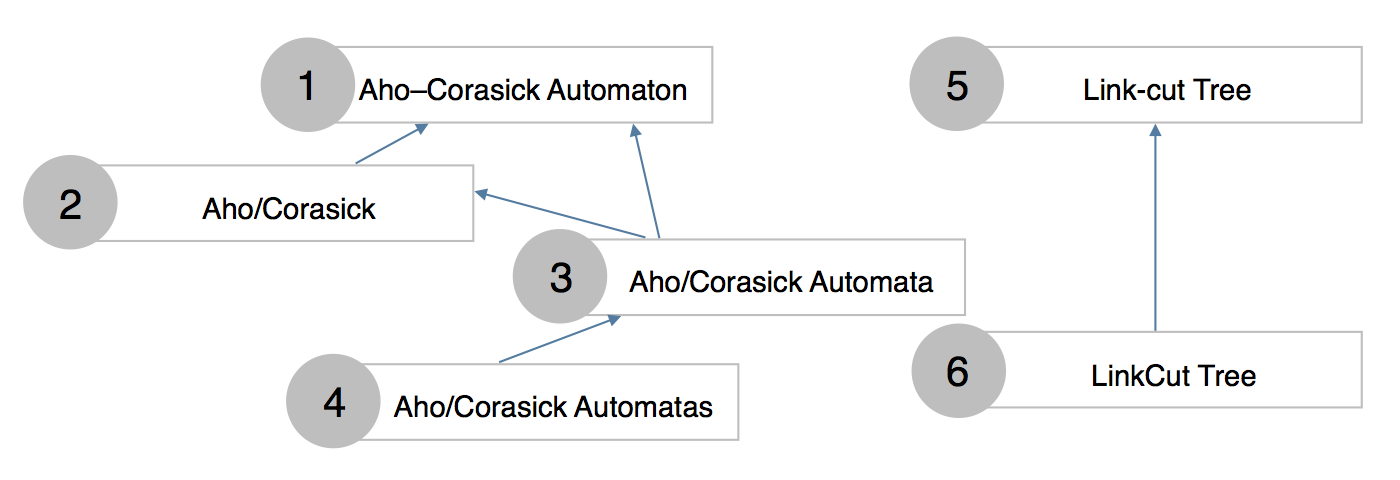
\includegraphics[scale=0.3]{image/cdag.png}
	\caption{DAG索引}\label{image:cdag}
\end{figure}

优化的方法并不复杂,只需要在前面的简单索引结构上加以改进。如果我们通过Hash将所有不同的$RME$对应为不同的数值,那么每个$RCS$就是一个数列。现在的问题变成了,要用已知的数列集合,压缩当前的数列。不难发现,这与之前的$comp$函数做的是同样的事情,仅仅是将字符串换成了数列。具体的过程也十分类似,只加了一步Hash转化,这里就不赘述了。\par
至此,我们已经完成了对索引结构的构建,实现了基本的压缩功能。下一章将介绍所需的数据结构,用于加速上述的算法过程。



\chapter{后缀自动机}
对于前面的压缩过程,需要在字符串集合中快速匹配模式串的最长前缀。而对于之后的k近似查询,也要找出模式串在集合中出现的所有位置。由于字符串的集合可以动态增加,所选取的数据结构必须能够动态维护。基于上述特性,虽然后缀树也可以满足需求,但本身结构较为复杂。因此,我们选择了较为简洁,却与后缀树\cite{ukkonen1995line}效果相同的后缀自动机\cite{ukkonen1993approximate}作为主要的数据结构。



\section{符号定义}
有限状态自动机是一种可以识别字符串的数据结构,对于一个自动机$A$,若它能识别字符串$s$,则记$A(s) = True$,否则$A(s) = False$。自动机由以下几部分构成:$\Sigma$为字符集,$State$表示状态集合,$Init$为初始状态,$End$为结束状态集合,$Trans$表示状态转移函数。用$trans(S, ch)$表示在状态$S$下读入字符$ch$后所达到的状态,同时令$trans(S, str)$表示在状态$S$下读入字符串$str$后所达到的状态。那么自动机$A$所能识别的字符串就是所有使得$trans(Init, s) \in End$的字符串$s$,记为$Reg(A)$。而从状态$S$开始能识别的字符串,即所有使得$trans(S, s) \in End$的字符串$s$,记为$Reg(S)$。



\section{算法原理}
顾名思义,关于字符串$s$的后缀自动机Suffix Automaton(简称$SAM$)是一个能识别$s$所有后缀的自动机,即$SAM(t) = True$当且仅当$t$是$s$的后缀。后面会介绍,$SAM$也能用于识别$s$所有的子串。这里,我们只关心最简状态后缀自动机,即状态数最少的自动机。后面会给出证明,它的复杂度是线性的。\par
对于最简状态后缀自动机$SAM$,我们用$ST(str)$表示$trans(Init, str)$,即从初始状态读入字符串$str$后达到的状态。对于字符串$s$,记它的后缀集合为$Suf$,子串集合为$Fac$。对于任何一个属于$Fac$的字符串$t$,$ST(t)$都对应一个合法的状态,因为可以在后面加入一些字符使其变成$s$的后缀。但我们不能将每个$t \in Fac$都对应一个状态,因为$Fac$的大小是$O(N^2)$的。考虑$ST(t)$所能识别的字符串集合$Reg(ST(t))$,对于$s$的后缀$x \in Suf$,如果$ST(t)$能识别$x$,则$t \circ x \in Suf$,即$Reg(ST(t))$是一些后缀集合。如果我们用$Right(t)$表示子串$t$出现的所有位置的右端点集合,那么$Reg(ST(t))$就完全由$Right(t)$决定。对于两个子串$u, v \in Fac$,如果$Right(u) = Right(v)$,则$ST(u) = ST(v)$。所以一个状态$S$对应所有$Right$集合等于$Right(t)$的字符串。\par
对于一个下标$r \in Right(t)$,只需要指定子串的长度$len$,就可以确定子串为$s(r - len, len)$。即给定一个状态的$Right$集合,只需要子串长度便可以确定子串。当给定的长度变短时,子串出现的位置可能变多,以至于超出$Right$集合的范围,但必然包含该$Right$集合。反之则得到$Right$集合的子集,我们将保证$Right$集合不变的子串长度范围记为$[Minl, Maxl]$。由此得出对于不同的状态,$Right$集合要么不相交,要么一个是另一个的真子集。不难发现,这种集合构成了树形的关系,我们称之为Parent树,如图\ref{image:partree}所示。\par

\begin{figure}[htbp]
	\centering
	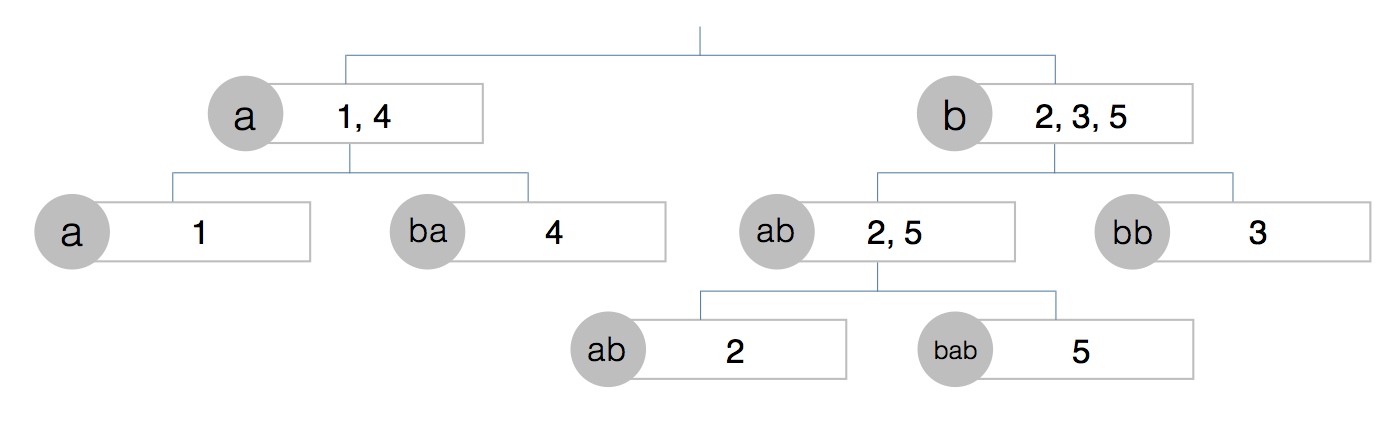
\includegraphics[scale=0.3]{image/partree.png}
	\caption{"abbab"的Parent树}\label{image:partree}
\end{figure}

不难发现,每个状态的$Right$集合都等于其孩子状态$Right$集合的并集,因此我们不必存下每个状态的$Right$集合,需要时通过深度优先搜索查询即可。同时也可以发现,对于长度范围,$Maxl(fa) = Minl(s) - 1$。\par
对于最长公共前缀的查询,我们只需要沿着状态转移函数走,直至走不到合法状态为止。从当前状态的$Right$集合中选出一个下标,结合转移步数,便可定位匹配的子串。而对于一般的字符串匹配,则必须将模式串全部走完,再递归求出整个$Right$集合,得到全部匹配的子串。\par
下面,我们来看如何动态构建$SAM$。



\section{动态构建}
由于需要满足动态扩展的特性,$SAM$的构建算法必须是在线的,即每次添加一个字符,并更新当前$SAM$使其成为包含该字符的$SAM$。\par
若当前字符串为$s$,长度为$l$,在加入字符$x$后,新增的子串必然是$s \circ x$的后缀。我们考虑所有表示$s$后缀的状态,对于其中的某个状态$p = ST(s)$,显然$p$对应的$Right$集合中有且只有一个$l$,而其他状态的$Right$集合都包含$l$,因此它们必然全是$p$的祖先。不妨将$p$沿着Parent树到根的路径记为$v_{1} = p, v_{2}, ... , v_{k} = root$。对于其中的一个状态$v$,它的$Right$集合为$\{r_{1}, r_{2}, ..., r_{n} = l\}$,那么在添加新字符$x$后形成的新状态$nv$中,只有$s[r_{i}] = x$的那些$r_{i}$是符合要求的。由此得出,如果从$v$出发没有标号为$x$的边(先不看$r_{n}$),那$v$的$Right$集合中就没有满足条件的$r_{i}$。如果从$v_{i}$出发有标号为$x$的边,由于$v_{i}$的$Right$集合是依次扩大的,那么$v_{i+1}$也有,因此我们考虑其中第一个有标号$x$的边的状态$v_{p}$。如果我们记添加字符$x$后的新状态$np = ST(s \circ x)$,则$Right(np) = \{l + 1\}$。对于$v_{p}$之前的状态,由于出发没有标号为$x$的边,其$Right$集合中只有$r_{n}$是满足要求的,因此将它们连一条到$np$标号为$x$的边。若$v_{p}$的$Right$集合为$\{r_{1}, r_{2}, ..., r_{n} = l\}$,记$trans(v_{p}, x) = q$,那么$q$的$Right$集合就是$\{r_{i} + 1 | s[r_{i}] = x\}$(注意这是更新前的情况,$r_{n}$是不算的)。但我们不能直接在$q$的$Right$集合中插入$l + 1$,因为以$l + 1$结尾的串可能达不到$Maxl(q)$的长度。当$Maxl(q) = Maxl(v_{p}) + 1$时不会有这种问题,令$Parent(np) = q$即可。否则需要新建节点$nq$,令$Right(nq) = Right(q) \cup \{l + 1\}$,此时的$Maxl(nq) = Maxl(v_{p}) + 1$,而$Right(q)$则是$Right(nq)$的真子集。所以令$Parent(q) = nq$,同时$Parent(np) = nq$即可。对于节点$nq$的状态转移函数$Trans(nq)$,由于$l + 1$后没有字符,所以与$Trans(q)$相同。最后,对于$v_{p}$之后的节点,只有连续的一段$v_{p}, ..., v_{e}$是会通过标号为$x$的边走到节点$q$的,由于节点$q$已经被替换成了$nq$,故只需要将$v_{p}, ..., v_{e}$的$trans(v_{i}, x)$设为$nq$即可。\par
至此,我们已经完成了对$SAM$的更新,流程如算法\ref{algo:samappend}所示。\par

\begin{algorithm}[H]
	\SetKwData{x}{x}\SetKwData{root}{root}\SetKwData{p}{p}\SetKwData{np}{np}\SetKwData{q}{q}\SetKwData{nq}{nq}
	\SetKwFunction{trans}{trans}\SetKwFunction{Parent}{Parent}
	\SetKwInOut{Input}{input}\SetKwInOut{Output}{output}
	\Input{$SAM$, character \x}
	\Output{new $SAM$}
	$Maxl(np) \leftarrow Maxl(p) + 1$\;
	\While{$\p \neq NULL\ And\ \trans{\p, \x} = NULL$}{
		$\trans{\p, \x} \leftarrow \np$\;
		$\p \leftarrow \Parent{\p}$\;
	}
	\If{$\p = NULL$}{
		$\Parent{\np} \leftarrow \root$\;
	}
	\uIf{$Maxl(\q) = Maxl(\p) + 1$}{
		$\Parent{\np} \leftarrow \q$\;
	}
	\Else{
		$\nq \leftarrow \q$\;
		$Maxl(\nq) \leftarrow Maxl(\p) + 1$\;
		$\Parent{\q} \leftarrow \Parent{\np} \leftarrow \nq$\;
		\While{$\p \neq NULL\ And\ \trans{\p, \x} = q$}{
			$\trans{\p, \x} \leftarrow \nq$\;
			$\p \leftarrow \Parent{\p}$\;
		}
	}
	\caption{Append character on SAM}\label{algo:samappend}
\end{algorithm}

可见,虽然原理上稍显复杂,但具体的算法流程还是很简洁的。



\section{线性证明}
$SAM$与后缀树相同,不管是空间复杂度,还是构造的时间复杂度,都是线性的。下面给出简单的证明。\par
观察Parent树可以发现,每个叶子节点都对应字符串的不同下标,因而叶子节点的个数只有N个。同时,由于每个内部节点至少有两个孩子,容易证明这棵树的大小必然是$O(N)$的。由于树上的每个节点代表一个$Right$集合,而$Right$集合又与状态一一对应。由此可知,$SAM$的状态数是线性的。\par
此外,我们还需要证明状态转移边的大小也是$O(N)$的。首先,SAM的状态和状态转移函数构成一张DAG,我们可以求出这个DAG的生成树(与Parent树没有关系),其根节点为$Init$,叶子节点为$End$。若状态数为$M$,则生成树上最多只有$M - 1$条边。而对于一条非树边$trans(S, c) = T$,我们构造$Init \rightarrow S$ -c-> $T \rightarrow End$的路径,其中$\rightarrow$表示生成树上的路径。由于这是一条从$Init$到$End$的路径,根据定义可知这条路径代表字符串的一个后缀。对于一个后缀,我们沿着自动机走,将其对应到经过的第一条非树边上,那么每个后缀最多对应一条非树边。而按照上面的方法构造,一条非树边至少可以被一个后缀所对应,所以非树边的数量不会超过后缀的数量。因此$SAM$的状态转移边数也是线性的。\par
综上可知,$SAM$的空间复杂度是线性的。而考察上面的在线更新算法可以发现,每插入一个字符,至多增加$np$与$nq$两个状态,因此构造$SAM$的复杂度也是线性的。


\section{具体应用}
通过后缀自动机,我们就可以快速构建上一章的索引结构了。\par
首先我们用一个$SAM$来维护$PREF$,对于需要加入到$PREF$中的字符串,只需将字符依次插入$SAM$中。为了防止匹配到的子串跨过多个主引用,还要在相邻的主引用间插入特殊的标识符。对于压缩过程,只需要用到最长公共前缀的查询,比较好的方式是在每个节点都记录一个$Right$集合中的值,这样就不用每次都递归下去寻找。同时,我们还要再用一个$SAM$来维护之前得出的$RCS$序列Hash值。对于初步压缩得到的$RCS$序列,利用同样的方式进一步压缩,然后将最终序列的哈希值依次插入到这一步的$SAM$中。在随后的k近似匹配中,还会用到$SAM$的模式匹配功能,这个将在下面介绍。\par
由于$SAM$的构造、查询复杂度都是线性的,所以通过$SAM$构建索引结构的复杂度等于读入字符串的长度和,即复杂度的下界。而$SAM$的空间复杂度同样也是线性的,从而保证了占用空间不超过$PREF$的长度和。由此可见,使用后缀自动机作为主要的数据结构是十分合适的。\par
接下来的章节,我们将介绍在索引结构中进行k近似匹配的方法。



\chapter{近似查询}
前面我们构建了基于多层次引用的索引结构,也介绍了如何使用后缀自动机将这一过程的复杂度降至最低。接下来,我们要讨论如何在索引结构中检索近似信息。



\section{k近似匹配}
在引言中我们说明了k近似匹配的规则,现在我们先介绍如何进行直观的k近似匹配,再介绍如何将其推广到索引结构中。\par
在经典的k近似匹配算法\cite{baeza1992fast}中,有一种称为种子扩展模式的方法。该算法基于这样一个事实:对于长度为$N$的模式串,如果文本串中存在与其编辑距离不超过k的子串,那么模式串与该子串之间必定存在长度至少为$r = \lfloor \frac{N}{k+1} \rfloor$的公共子串。基于这一性质,我们可以先将模式串等分成$k + 1$份种子,对于每个种子先找出它在文本串中的精确匹配。假设匹配位置的下标为$i$,根据编辑距离的特性,近似匹配的结果必然在$[i - (N - r) - k, i + N + k]$这一区间中,之后的求解可以分不同情况使用Shift-or、Bit-parallel等算法。由于该部分可以细分许多情况,十分复杂,在这里我们直接使用滚动数组优化的动态规划算法求解。\par
对于某个种子找出的精确匹配位置$i$,我们与种子前面的模式串$pre$做逆向(从右向左)的动态规划,记录下区间$[i - (N - r) - k, i]$中各个位置到$i$的子串与$pre$的编辑距离结果。再从$i + r$开始与种子后面的模式串$suf$做正向的动态规划,通过类似的过程记录下结果。由于动态规划的转移至多与前一列有关,而我们只关心最后一列的结果,因此可以利用滚动数组将空间降至$O(N)$,如图\ref{image:dp}所示。将上面两步得出的结果排序后扫描,便可快速得出所有k近似匹配子串。\par

\begin{figure}[htbp]
	\centering
	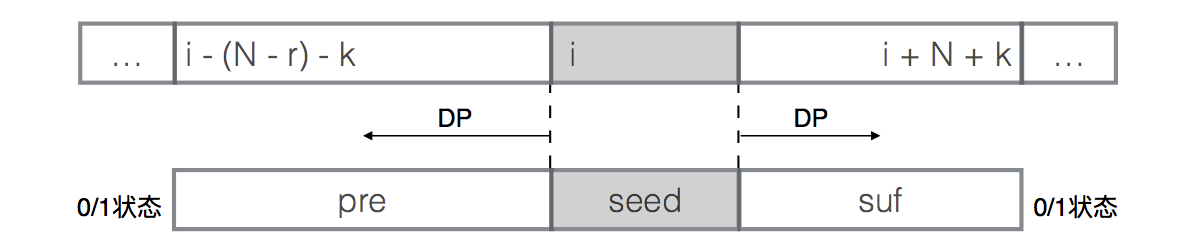
\includegraphics[scale=0.35]{image/dp.png}
	\caption{动态规划}\label{image:dp}
\end{figure}

以上算法的基础在于,能够在字符串集合中快速精确匹配种子出现的所有位置。幸运的是,后缀自动机完全可以胜任,具体方法之前也已提到。因此,对于索引结构上的k近似匹配,可以先在$PREF$构成的后缀自动机上匹配种子出现的位置,再在主引用中通过动态规划找出全部的k近似匹配。但这样得到的只是$PREF$中的结果,如何将其扩展到$COMP$集合上呢?我们将在下一节解决这个问题。



\section{区间覆盖与区间树}
上一节我们完成了在$PREF$中的k近似匹配,对于其中的某个匹配结果,实质上是一个主引用的子串。如果其他串的某个索引刚好覆盖这一子串,则该结果也必然出现在那个串中。基于这一逻辑,对于$refid$相同的一些$RME$,他们对应的区间存在一定的覆盖关系。如果我们能维护这种覆盖关系,就能从$PREF$中的结果开始,通过宽度优先搜索的方式推出全部$COMP$中的结果。\par
那我们该如何维护这种关系呢?显然,区间树\cite{cormen2009introduction}是个很好的选择。\par
区间树是一种基于平衡树的数据结构。我们都知道,平衡树可以快速维护有序序列,在$O(logN)$的复杂度下完成元素的插入、删除,序列的最值查询等。而区间树则可以维护区间集合及其内部关系,除了可以快速插入、删除区间外,还可以找出覆盖某个区间的所有区间子集,而后者刚好是我们所需要的。图\ref{image:intvtree}展示了区间树的组织形式。\par

\begin{figure}[htbp]
	\centering
	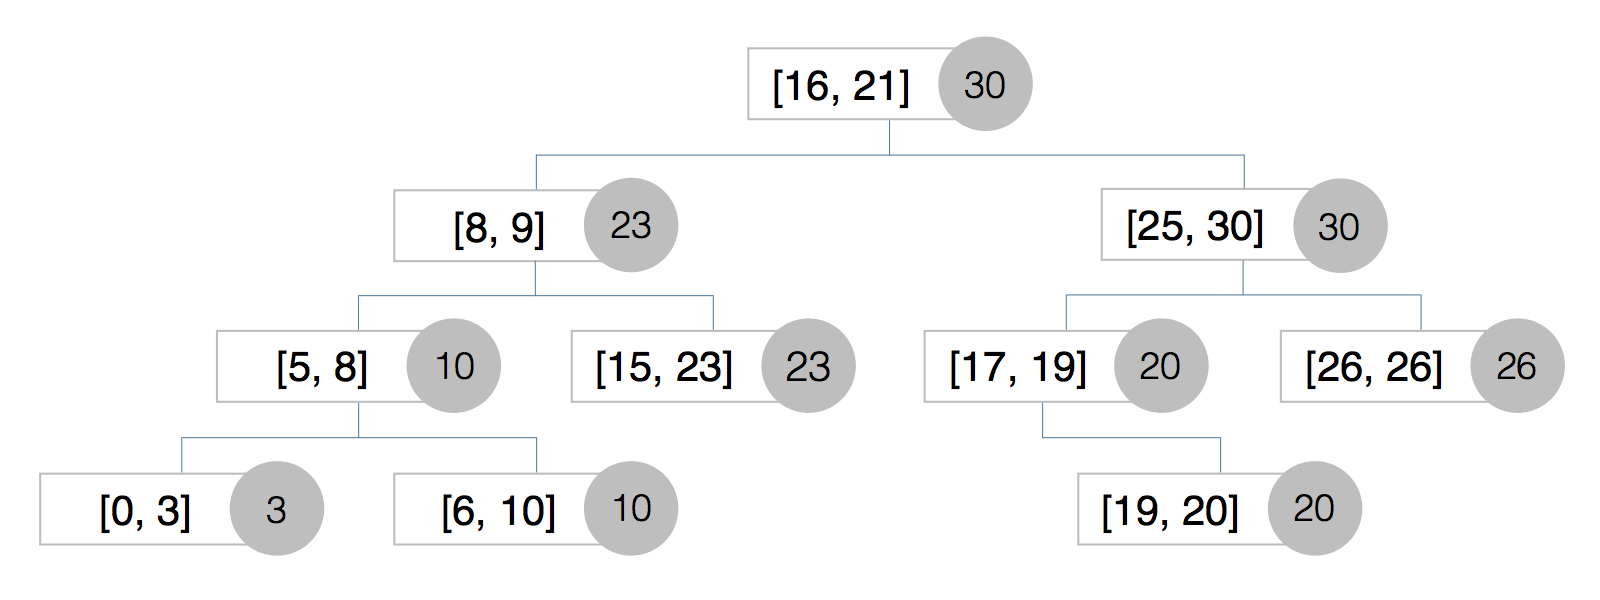
\includegraphics[scale=0.25]{image/intvtree.png}
	\caption{区间树}\label{image:intvtree}
\end{figure}

从图中可以看到,每个区间以一个节点的方式出现在平衡树中,而区间的左端点则用来作为比较的键值。值得注意的是,每个节点除了记录区间的右端点外,还记录了当前子树下右端点的最值。这样的好处在于,对于查询要覆盖的区间$[s, t]$,如果该子树下最右的端点都小于$t$,那么这棵子树中一定不存在可行解。\par
由此,我们得出在区间树中查询所有覆盖区间$[s, t]$节点的算法。首先从区间树的根节点$root$开始进行深度优先搜素,如果当前节点对应子树的右端点最值小于$t$则直接返回。否则比较该节点的左端点与$s$的大小关系,如果左端点小于等于$s$,则检查该点是否为可行答案,然后同时递归进入两棵子树中,否则只递归进入左子树。流程如算法\ref{algo:intquery}所示,其中$low$表示左端点,$high$表示右端点,$maxh$表示子树中右端点的最值,左右子树分别用$left$与$right$表示。\par

\begin{algorithm}[H]
	\SetKwData{u}{u}\SetKwData{s}{s}\SetKwData{t}{t}\SetKwData{root}{root}\SetKwData{result}{result}
	\SetKwFunction{dfs}{dfs}\SetKwFunction{low}{low}\SetKwFunction{high}{high}\SetKwFunction{maxh}{maxh}\SetKwFunction{left}{left}\SetKwFunction{right}{right}
	\SetKwProg{Procedure}{Procedure}{}{}
	\SetKwInOut{Input}{Input}\SetKwInOut{Output}{Output}
	\Input{\root of IntTree, interval [\s, \t]}
	\Output{set of Node which cover interval [\s, \t]}
	\Procedure{\dfs{\u, \s, \t}}{
		\If{$\u = NULL\ Or\ \maxh{\u} < \t$}{
			return
		}
		\If{$\low{\u} \leq \s$}{
			\If{$\high{\u} \geq \t$}{
			add \u to \result}
			\dfs{\right{u}, \s, \t}\;
		}
		\dfs{\left{u}, \s, \t}\;
	}
	\caption{Query interval in IntTree}\label{algo:intquery}
\end{algorithm}

至此,我们可以对每个字符串都建一棵区间树,用以维护引用该字符串的索引。然后将$PREF$中的结果插入宽度优先搜索队列中,每次取出队头的结果,在它对应的区间树中找出所有覆盖该区间的$RME$,通过$RME$的$offset$计算出结果对应的子串,再将该子串插入搜索队列中,重复上述过程即可。由于区间树的空间复杂度是$O(N)$的,因此最终占用的空间不会超过所有$RCS$大小的总和。



\section{重叠时的匹配}
经过前面的步骤,我们已经完成了大部分结果的匹配,但还有一小部分的遗漏。如果$COMP$中的结果跨越不止一个$RME$,只考察区间覆盖的话并不能涉及这种情况。因此我们还需要最后一步,找出跨越$RME$交点的匹配结果。\par
如果模式串的长度最多为$maxn$,而询问的误差最多为$maxk$,由于编辑距离的特性,令$\delta = maxn + maxk - 1$,则跨越$RME$的结果必然在以$mismatch$为中心的长度为$\delta * 2 + 1$的区间内。
我们可以再用一个$SAM$来维护每个$RME$对应区间里的字符串,和$PREF$一样将它们全部连接起来插入$SAM$中,称为$OVLP$,然后像之前的过程一样进行查询即可。需要注意的是,在$RME$长度较短而$\delta$较大时这些区间可能会重叠,重复插入会浪费空间与构造速度,插入时跳过已经插入的前缀即可。下面我们以2.3节中的例子作为演示:\par



\section{样例演示}
这里我们令$maxn = 3$,$maxk = 1$,检索的模式串为"ivk"。\par
\begin{itemize}
	\item 首先我们将模式串按照规则划分为两个种子:"i"与"vk",由于"vk"在所有字符串中都没有精确匹配,这里我们只考虑关于"i"的结果。
	\item 接着我们在$PREF$中进行匹配,对于$s_{1}$我们精确匹配"i"后得到"ick"满足条件,而在$s_{5}$中则匹配到"ink"。故当前的答案\\
		$result = \{(s_{1}, 9, 3, "ick"), (s_{5}, 1, 3, "ink")\}$
	\item 然后在$OVLP$中进行匹配,此时的$OVLP$为\\
		aton|Aho/Cora|sick|Aho/Cora|mata|matas|Tree|inkCut Tree\\
		找到$s_{2}$中的"ick"与$s_{6}$中的"ink",当前答案\\
		$result = \{(s_{1}, 9, 3, "ick"), (s_{2}, 9, 3, "ick"), (s_{5}, 1, 3, "ink"), (s_{6}, 1, 3, "ink")\}$
	\item 最后要在区间树中搜索答案。$s_{1}$对应的区间树如图\ref{image:intvtree1}所示,查询区间$[9, 11]$找到$s_{3}$中的$[4, 19]$。之后根据$s_{2}$的区间树得出$s_{4}$中的区间$[0, 19]$,根据$s_{5}$的区间树找出$s_{6}$的区间$[0, 3]$。至此得出所有的覆盖区间,结合$RME$的$offset$得到最终答案\\
		$result = \{(s_{1}, 9, 3, "ick"), (s_{2}, 9, 3, "ick"), (s_{3}, 9, 3, "ick"),\\
		{\qquad \qquad}(s_{4}, 9, 3, "ick"), (s_{5}, 1, 3, "ink"), (s_{6}, 1, 3, "ink")\}$
\end{itemize}

\begin{figure}[htbp]
	\centering
	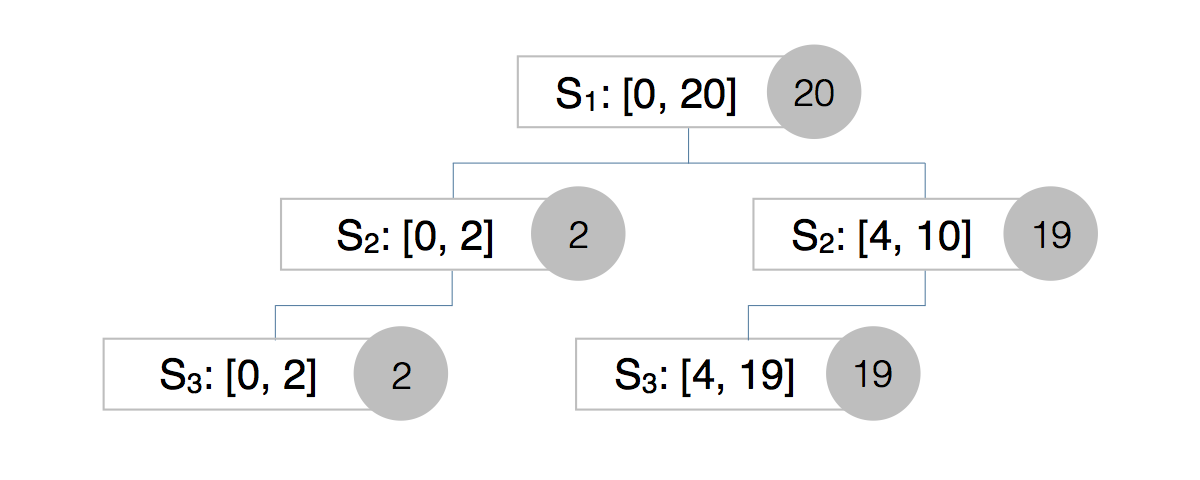
\includegraphics[scale=0.35]{image/intvtree1.png}
	\caption{$s_{1}$的区间树}\label{image:intvtree1}
\end{figure}

至此我们已经完成了在索引结构中进行k近似匹配的所有步骤,总结起来分以下三步:1)在主引用中利用$SAM$与动态规划匹配结果;2)通过与第一步类似的方式找出$COMP$中跨越$RME$的结果;3)通过区间树将之前的结果扩展到$RME$内部的结果。需要注意的是,第二步与第三步不能交换,因为跨过$RME$的结果可能被某个索引完全覆盖。



\chapter{实验结果}
实验的部分,我们将分别以DNA突变序列与Wiki百科历史版本作为实验数据,考察算法的压缩效率及检索速度。同时,通过数据量与压缩速度、压缩率的关系,考察算法是否为线性复杂度。



\section{实验平台及编译环境}
本次实验的实验平台为OSX 10.11.4,CPU工作频率2.4GHz,内存8GB,编译器为Apple LLVM 7.3.0 (clang-703.0.29)。



\section{DNA突变序列}
这里我们选取了人类基因组计划的染色体文本数据,对每条染色体取其前1,000行DNA序列,随后模拟自然环境下的变异、交叉互换等规则,生成一系列基因突变后的DNA序列。对数据进行压缩后,检索DNA片段"ATCGATCGG"在误差$k = 1$时出现的所有位置,结果如表格\ref{tab:dnacompress}所示。\par

\begin{longtable}{crrrrrr}
	\caption{关于基因突变序列的压缩结果}\label{tab:dnacompress}\\
	\hline\hline
	染色体编号 & 迭代次数 & 数据集大小 & 压缩时间 & 压缩率 & 检索时间 & 匹配数 \\
	\hline
	\endfirsthead
	\multicolumn{7}{r}{续表\ref{tab:dnacompress}}\\
	\hline\hline
	染色体编号 & 迭代次数 & 数据集大小 & 压缩时间 & 压缩率 & 检索时间 & 匹配数 \\
	\hline
	\endhead
	\hline
	\endfoot
	\hline
	\endlastfoot
	3501 & 256 & 12.18MB & 3.30s & 7.07\% & 0.00s & 56 \\
	3501 & 4096 & 200.54MB & 105.02s & 7.63\% & 2.02s & 11137 \\
	3502 & 256 & 12.18MB & 3.30s & 5.65\% & 0.01s & 294 \\
	3502 & 4096 & 200.34MB & 84.67s & 5.70\% & 3.43s & 10239 \\
	3503 & 256 & 12.18MB & 3.31s & 6.02\% & 0.00s & 0 \\
	3503 & 4096 & 200.54MB & 72.17s & 4.54\% & 1.21s & 2111 \\
	3504 & 256 & 12.18MB & 3.50s & 7.35\% & 0.00s & 0 \\
	3504 & 4096 & 200.37MB & 98.26s & 6.70\% & 2.63s & 7448 \\
	3505 & 256 & 12.18MB & 3.83s & 8.20\% & 0.00s & 404 \\
	3505 & 4096 & 200.36MB & 106.59s & 7.63\% & 0.97s & 7340 \\
	3506 & 256 & 12.18MB & 3.42s & 6.62\% & 0.00s & 266 \\
	3506 & 4096 & 200.56MB & 91.50s & 6.27\% & 2.38s & 11455 \\
	3507 & 256 & 12.18MB & 3.77s & 7.86\% & 0.00s & 305 \\
	3507 & 4096 & 200.42MB & 106.08s & 7.72\% & 3.43s & 13525 \\
	3508 & 256 & 12.18MB & 2.90s & 4.64\% & 0.00s & 51 \\
	3508 & 4096 & 200.36MB & 64.84s & 4.24\% & 1.38s & 5620 \\
	3509 & 256 & 12.18MB & 3.25s & 6.91\% & 0.00s & 412 \\
	3509 & 4096 & 200.37MB & 86.38s & 6.03\% & 1.83s & 16015 \\
	3510 & 256 & 12.18MB & 3.60s & 7.01\% & 0.00s & 511 \\
	3510 & 4096 & 200.28MB & 103.80s & 7.40\% & 3.13s & 9758 \\
	3511 & 256 & 12.18MB & 3.70s & 7.43\% & 0.01s & 209 \\
	3511 & 4096 & 200.53MB & 103.73s & 7.32\% & 1.99s & 6674 \\
	3512 & 256 & 12.18MB & 3.17s & 5.05\% & 0.00s & 250 \\
	3512 & 4096 & 200.34MB & 82.98s & 5.74\% & 2.24s & 17235 \\
	3513 & 256 & 12.21MB & 0.38s & 0.92\% & 0.00s & 0 \\
	3513 & 4096 & 207.52MB & 5.00s & 0.12\% & 0.00s & 0 \\
	3514 & 256 & 12.21MB & 0.38s & 0.92\% & 0.00s & 0 \\
	3514 & 4096 & 207.52MB & 5.03s & 0.12\% & 0.00s & 0 \\
	3515 & 256 & 12.18MB & 3.58s & 7.05\% & 0.00s & 34 \\
	3515 & 4096 & 200.35MB & 99.40s & 6.86\% & 2.37s & 11209 \\
	3516 & 256 & 12.18MB & 3.57s & 8.42\% & 0.00s & 814 \\
	3516 & 4096 & 200.57MB & 111.26s & 8.25\% & 3.32s & 25034 \\
	3517 & 256 & 12.18MB & 3.87s & 8.41\% & 0.00s & 0 \\
	3517 & 4096 & 200.28MB & 121.32s & 8.26\% & 5.56s & 19668 \\
	3518 & 256 & 12.18MB & 3.36s & 6.41\% & 0.00s & 508 \\
	3518 & 4096 & 200.51MB & 78.89s & 5.54\% & 0.76s & 5907 \\
	3519 & 256 & 12.18MB & 4.02s & 8.77\% & 0.00s & 256 \\
	3519 & 4096 & 200.45MB & 117.96s & 8.38\% & 1.26s & 7725 \\
	3520 & 256 & 12.18MB & 3.53s & 6.50\% & 0.00s & 254 \\
	3520 & 4096 & 200.36MB & 93.47s & 6.52\% & 0.59s & 7660 \\
	3521 & 256 & 12.21MB & 0.50s & 0.92\% & 0.00s & 0 \\
	3521 & 4096 & 207.52MB & 7.03s & 0.12\% & 0.00s & 0 \\
	3522 & 256 & 12.21MB & 0.40s & 0.92\% & 0.00s & 0 \\
	3522 & 4096 & 207.52MB & 5.77s & 0.12\% & 0.00s & 0 \\
	3523 & 256 & 12.18MB & 3.59s & 8.15\% & 0.00s & 507 \\
	3523 & 4096 & 200.51MB & 114.35s & 8.26\% & 2.41s & 14108 \\
	3524 & 256 & 12.18MB & 3.54s & 7.03\% & 0.01s & 512 \\
	3524 & 4096 & 200.08MB & 90.57s & 6.33\% & 3.56s & 18422 \\
\end{longtable}

从上表可以看出,对于200MB左右的数据,算法的压缩率在5\%到8\%左右,压缩耗时约100秒。而对于检索来说,大约可在2秒左右检索出10,000条结果。其中13、14、21与22号染色体的结果比较特别,压缩率都在1\%以下。这是因为以上几条染色体的前1,000行DNA序列都为空,也刚好说明了对于重复率越高的数据,压缩效率就越高。\par
对于前4条染色体,我们分别制作了压缩时间与压缩率关于数据规模的图表,如图\ref{fig:cchart}所示。\par

\begin{figure}[htbp]
	\centering
	\subfloat[压缩时间]{
		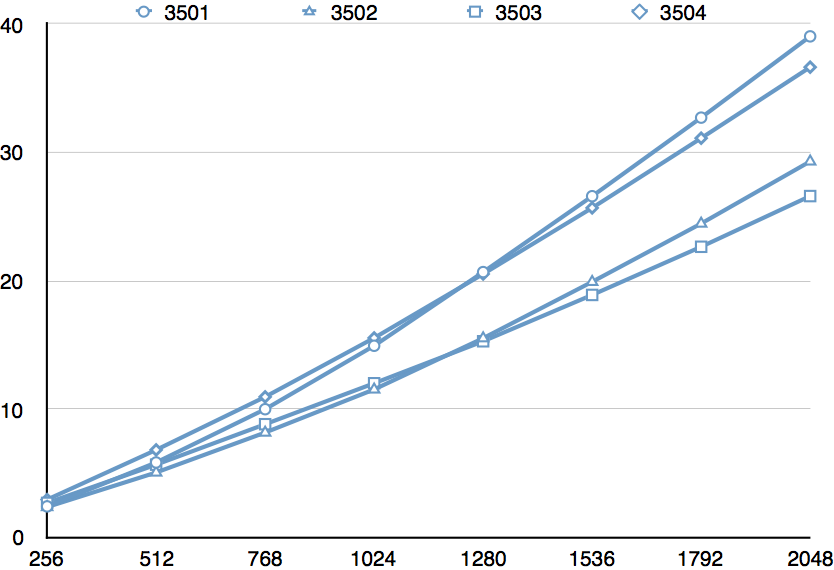
\includegraphics[scale=0.85]{image/ctime.png}
	}\\
	\subfloat[压缩率]{
		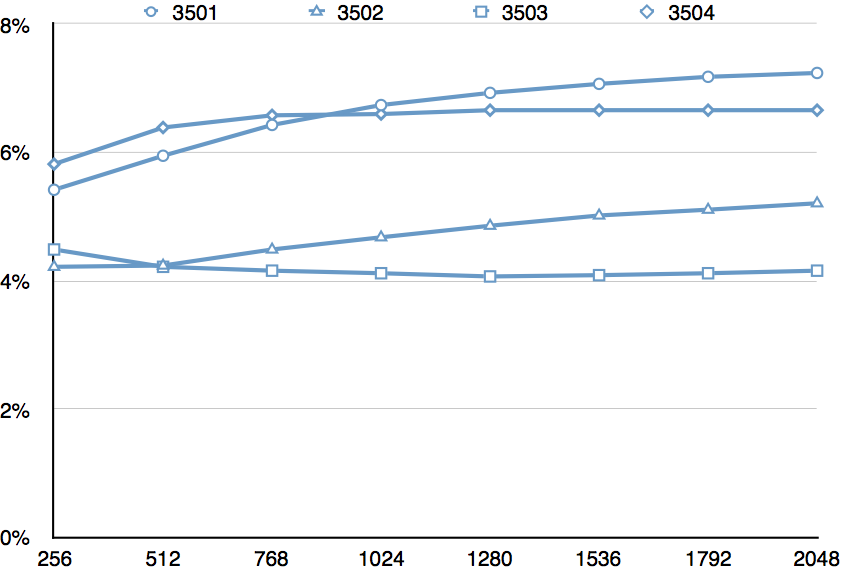
\includegraphics[scale=0.85]{image/cratio.png}
	}
	\caption{压缩效果与数据规模的关系}\label{fig:cchart}
\end{figure}

从图表中可以看出,压缩时间与数据规模之间保持线性关系,而压缩率则基本不变。



\section{Wiki历史版本}
本节我们选取了Wiki百科部分词条的历史版本列表,考察对于文本文档数据的压缩效果。对于每个词条,我们分别选取了最近20条与最近100条历史记录,结果如表格\ref{tab:wikicompress}所示。\par

\begin{longtable}{crrrrrr}
	\caption{Wiki历史文档的压缩结果}\label{tab:wikicompress}\\
	\hline\hline
	Wiki词条 & 数据集大小 & 压缩时间 & 压缩率 & 模式串及误差 & 检索时间 & 匹配数 \\
	\hline
	\endfirsthead
	\multicolumn{7}{r}{续表\ref{tab:dnacompress}}\\
	\multicolumn{7}{c}{(接上页)}\\
	\hline\hline
	Wiki词条 & 数据集大小 & 压缩时间 & 压缩率 & 模式串及误差 & 检索时间 & 匹配数 \\
	\hline
	\endhead
	\hline
	\multicolumn{7}{c}{(接下页)}
	\endfoot
	\hline
	\endlastfoot
	Asimov & 1.65MB & 0.40s & 11.50\% & "Robot" 2 & 0.20s & 14740 \\
	Asimov & 8.16MB & 1.65s & 8.37\% & "Asiimov" 1 & 0.87s & 38912 \\
	AWP & 0.58MB & 0.15s & 17.00\% & "Kill" 2 & 0.79s & 16554 \\
	AWP & 2.80MB & 0.79s & 13.91\% & "Sniper" 1 & 0.11s & 6260 \\
	Warcraft & 0.43MB & 0.12s & 14.12\% & "Night" 2 & 0.00s & 2220 \\
	Warcraft & 2.04MB & 0.53s & 11.87\% & "Elf" 1 & 0.00s & 1410 \\
	JangJaeho & 0.38MB & 0.11s & 15.25\% & "Spirit" 2 & 0.00s & 640 \\
	JangJaeho & 1.84MB & 0.46s & 12.13\% & "Moon" 1 & 0.78s & 10540 \\
	ICPC & 0.32MB & 0.09s & 19.01\% & "Final" 2 & 1.27s & 17044 \\
	ICPC & 1.49MB & 0.36s & 15.06\% & "China" 1 & 0.03s & 3340 \\
	Algorithm & 1.59MB & 0.44s & 13.09\% & "KMP" 2 & 0.15s & 24265 \\
	Algorithm & 7.99MB & 1.79s & 9.17\% & "Match" 1 & 0.00s & 3914 \\
\end{longtable}

从实验结果中可以看出,对于比DAN序列更加复杂的文本文档,该算法的压缩时间与检索时间基本保持不变。而压缩率则略有下降,约在8\%到20\%之间。总体来说来说,该算法对于文本文档依然有着优秀的压缩速度与压缩率,也保持了高速的近似检索能力。



\chapter{结论}
本文首先表述了字符串压缩与检索相结合的技术在当下的实际意义,然后介绍了字符串压缩的具体思路——基于多引用的层次化索引结构。为了解决压缩过程中需要的字符串集合中的模式匹配问题,也为之后的k近似匹配打下基础,我们引入了一种简洁的数据结构——后缀自动机,并介绍了它的算法原理及构造方式。由于后缀自动机的复杂度是线性的,因此保证了构造的时间与最终的空间开销与读入规模一致。在之后我们介绍了利用后缀自动机进行k近似匹配的方式,并通过区间树与特殊情况的处理,将匹配扩展到整个索引结构中,从而实现了近似检索的功能。最后我们通过对DNA突变序列及Wiki百科历史文档的实验,验证了算法的压缩速度、压缩率及检索速度,并考察了算法复杂度与数据规模的线性关系,证明了算法的有效性及高效性。\par
但该算法也有一定的不足之处:1)虽然做到了动态查询,支持边插入边查询的功能,但无法完成对字符串集合的删除及修改等操作;2)由于最优索引结构是NP问题,本文只提出了一个基于贪心策略的较优的构建方式,没有探究更优的策略;3)在基于后缀自动机的k近似匹配中,仅使用了滚动数组优化的动态规划算法,还有改进的空间;4)区间数与边界情况的处理复杂度略高,需要更优的数据结构进行优化等。对于上述的不足,还有待以后的研究与改进。\par
最后,后缀树作为处理字符串模式匹配的经典方式,已经得到了广泛的应用。而与之功能相仿的后缀自动机,则拥有更简洁的实现方式,在诸如子串计数等问题上甚至有着更优的表现。可见,发挥数据结构对于不同问题的能力,对算法的优化方面很有意义。



\zihao{-5}\songti
\bibliographystyle{sysuthesis}
\bibliography{main}

\appendix

\begin{thankto}
	\songti\zihao{-4}
	首先,我要对林瀚老师表示衷心的感谢。老师的细心指导,使我渐渐熟悉字符串压缩匹配这一陌生的领域,提出了很多宝贵的建议,对整个毕业设计的完成提供了很大的帮助。老师治学态度严谨,从选题、方法研究、提纲到论文整个过程都严格把关,对我的求学态度产生了深深的影响。\par
	感谢本科阶段的所有教育和帮助过我的老师们,你们的认真讲解与耐心指导为我的科研活动打下了坚实的基础。\par
	感谢集训队的马研奋、张健昶同学的帮助与指导,在我遇到困难的时候能够提出有效的建议。\par
	感谢陈晓燕同学,在论文的撰写过程中给了我很大的帮助,让我受益良多。\par
	我还要感谢我的父母和家人,在学习和生活上给予我莫大的关心与支持。\par
	最后,我要感谢其他在这个领域的相关研究人员,你们的工作成果给予了我很大的启示。谢谢你们!

	\vskip 18pt
	\begin{flushright}
		李贝瑀\\
		\today
	\end{flushright}
\end{thankto}

\backmatter

\end{document}
